\chapter{PMLSM design with Harmonics Modelling technique}   \label{Chapter:PMLSM design HM}


    Previously explored by Ruddy et al. \cite{Ruddy2015}, \acsp{PMLSM} or more precisely tubular, slotless, permanent magnet excited, longitudinal flux, and linear 3-phase motors have shown superior potential when compared to \acsp{VCM} in \acs{NFJI} applications. The scaling laws for \acsp{PMLSM} allow the overall system to operate a magnitude higher efficiency. The potential of a better actuator for \acs{NFJI} has been proven with \acsp{PMLSM}, accompanied with computationally efficient, exact semi-analytical magnetic field \acsp{HM} solution. However, large efficiency gain is only possible if the total length of motor is allowed to be very long which will be impractical for fitting in an actual injector device. An appropriate optimization scheme with the necessary constraints will be required to not only realize a practical actuator for \acs{NFJI}, but flexible enough to compare with other types of \acsp{LSDDM} in existence.
    
    
    This chapter considers the requirements tailored to \acs{NFJI} to describe a modified design of \acs{PMLSM} from that already presented in \cite{Ruddy2015}. Then, an universal optimization scheme for \acsp{LSDDM} with fixed maximum motor length, motor mass, and input power dissipation is presented. This optimization method helps determining a \acs{PMLSM} motor design that produce the fastest water jet injection velocity with the given constraints. 


% ===================================================================================================
% === NEW SECTION === NEW SECTION === NEW SECTION === NEW SECTION === NEW SECTION === NEW SECTION ===
% ===================================================================================================
\section{Electromagnetic model}                 \label{Chapter:PMLSM design HM/electromagnetic model}


    % -----------------------------------------------------------------------------------
    % --- NEW SUB SECTION --- NEW SUB SECTION --- NEW SUB SECTION --- NEW SUB SECTION --- 
    % -----------------------------------------------------------------------------------
    \subsection{Scaling model}                  \label{Chapter:PMLSM design HM/electromagnetic model/scaling}


        \begin{figure*}[ht]
          \centering
          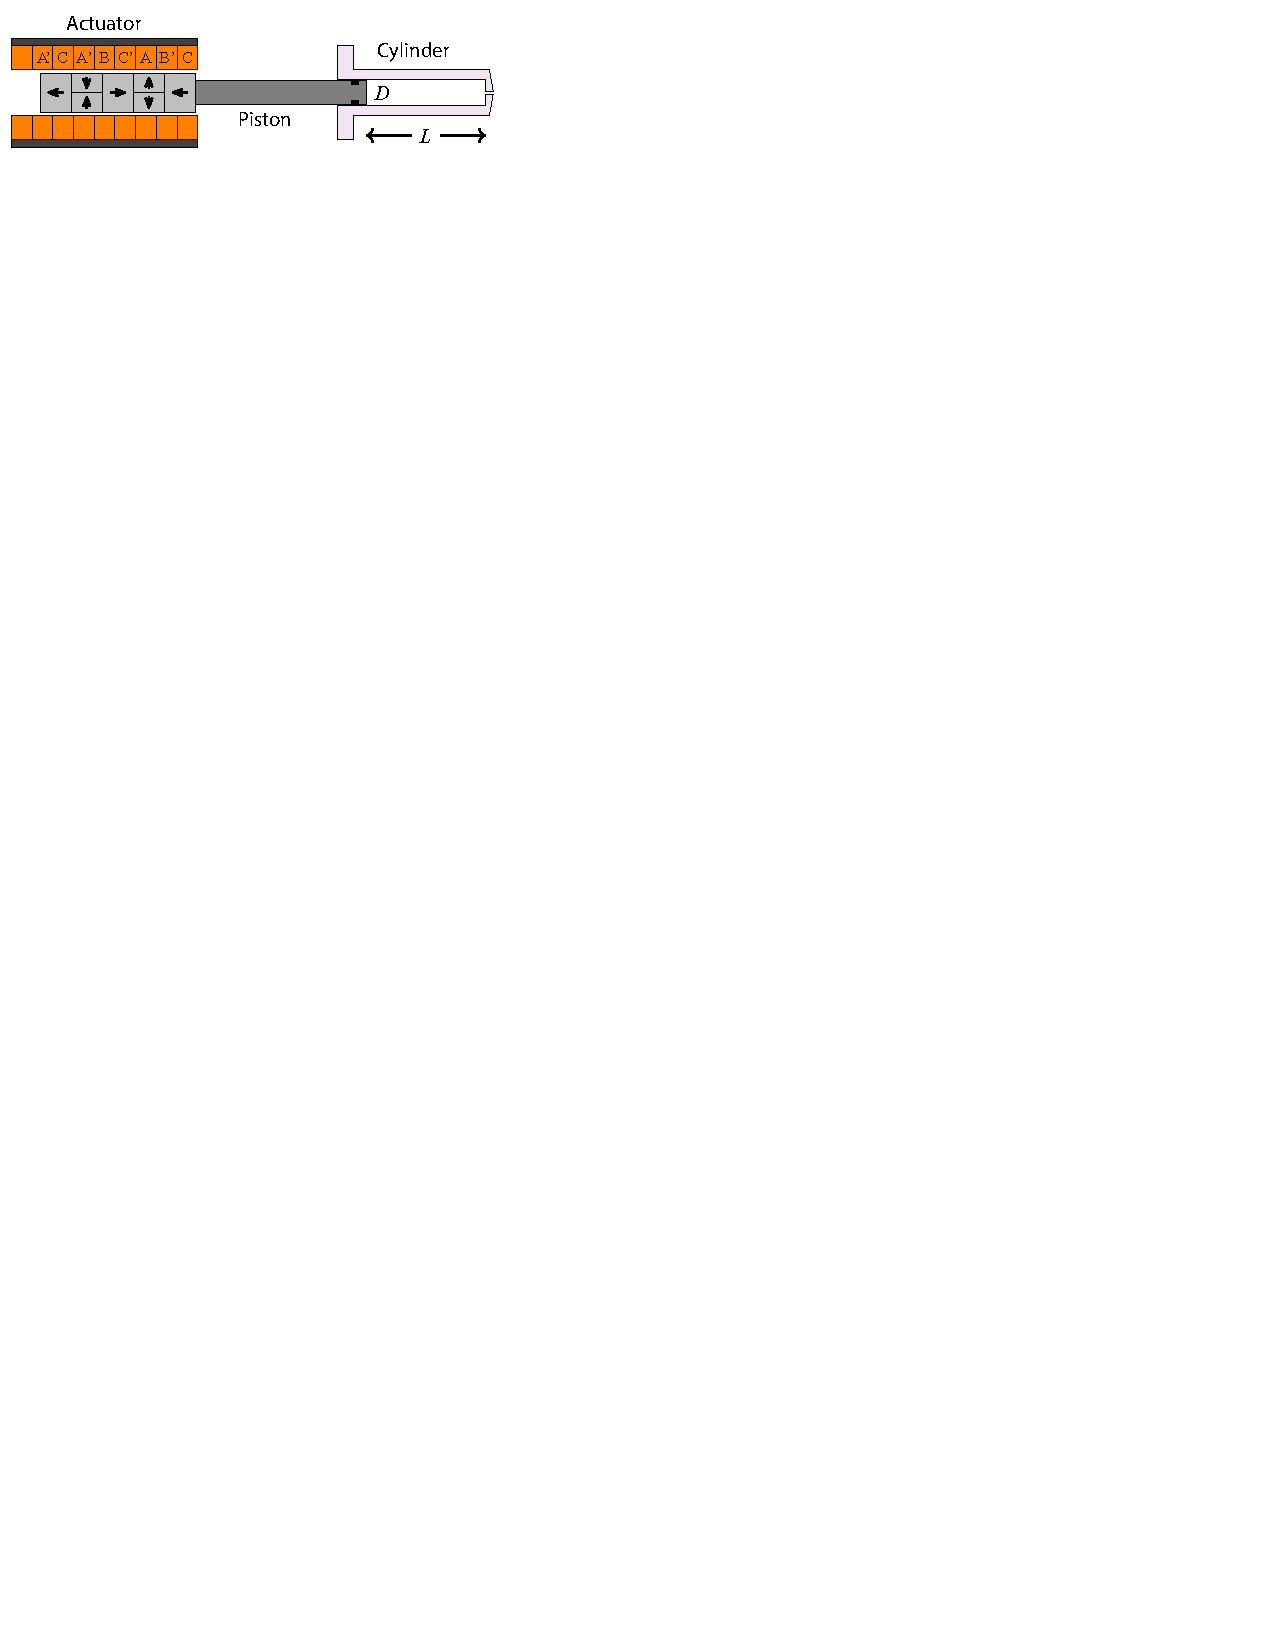
\includegraphics[width=0.7\textwidth]{chap3/images/PMLSM_scaling_law_illustration.pdf}
          \caption{A basic schematic of a synchronous motor, driving a jet injector. Ampoule diameter $D$ and piston stroke $L$ are illustrated.}
          \label{fig:chapter/hm/PMLSM scaling law illustrated}
        \end{figure*}


        Ignoring resistance due to fluid viscosity and atmospheric pressure, due to Bernoulli's equation for an incompressible and steady fluid flow, the actuator force $F$ and jet speed $v_{jet}$ have the following relation:
        
        
        \begin{equation}
            F=\frac{\pi}{8}\rho_w {v_{jet}}^2 D^2
            \label{eq:actuation force by PMLSMs}
        \end{equation}
        
        
        where $\rho_w$ is the density of fluid being delivered and $D$ is the diameter of the piston cylinder. For linear permanent magnet motors, the motor constant $K_m$, measured in $\mathrm{N/\sqrt{W}}$, is a measurement of force production efficiency that is independent of the winding properties. We can combine these relationships to find the power dissipation in the motor windings $P$ for a given ampoule volume $V$ and length of piston travel $L_s$:


        \begin{equation}
            P=\frac{\rho^2V^2{v_{jet}}^4}{4{K_m}^2 L_s^2}
            \label{eq:power dissipation for PMLSMs}
        \end{equation}
        
        
        It was shown in \cite{Ruddy2011a} that $K_m \propto {\hat K}_m \sqrt M$, where ${\hat K}_m$ is a dimensionless parameter describing the internal magnetic and electric geometry of the motor. Thus, neglecting material properties, we can determine the overall scaling behavior of motors for the needle free jet injection task:
        
        
        \begin{equation}
            P\propto\frac{V^2v^4}{ {M L_s^2{\hat K^2}_m} }
            \label{eq:scaling law for PMLSMs}
        \end{equation}
        
        
        Typically the application determines $\rho$, $V$, $v$, and $L_s$ (or $D$). Thus, either motor mass $M$ must be fixed to search for a motor with the optimum power consumption $P$, or $P$ must be fixed to find a motor with the optimum motor mass.


    % -----------------------------------------------------------------------------------
    % --- NEW SUB SECTION --- NEW SUB SECTION --- NEW SUB SECTION --- NEW SUB SECTION --- 
    % -----------------------------------------------------------------------------------
    \subsection{Topology}                       \label{Chapter:PMLSM design HM/electromagnetic model/topology}
    
    
        \begin{figure*}[ht]
          \centering
          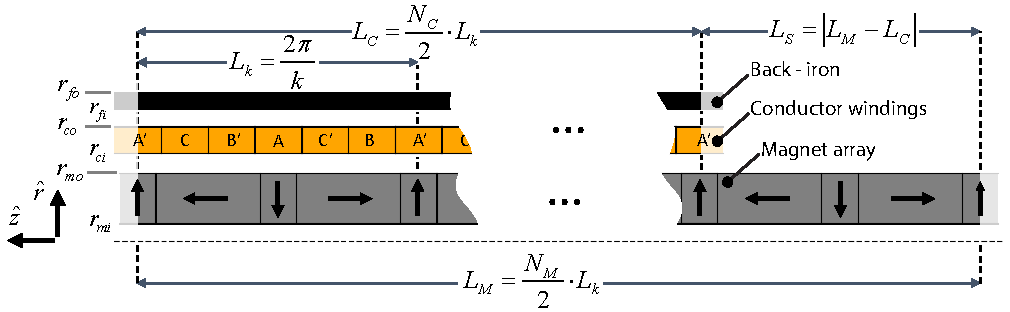
\includegraphics[width=5.8in]{chap3/images/PMLSM.pdf}
          \caption{This schematic illustrates a tubular LPMSM with quasi-Halbach magnets, slotless windings, and a shortened exterior back-iron tube. The radii of magnet, coil, and back are shown; the structure has periodicity with wave number $k$, wave length $L_k$, number of half coil poles $N_C$ and half magnet poles $N_M$. The arrows indicate direction of magnetization of magnets, while the characters label the coil phases.}
          \label{fig:chapter/hm/PMLSM motor construction fullpage}
        \end{figure*}
    
        
        Based on \cite{ruddy2014}, we will study a slight variation of this topology using a shorter exterior back-iron. In this approach, the back-iron only covers the coil and travels along with it, as shown in Fig.~\ref{fig:chapter/hm/PMLSM motor construction fullpage}. The advantage of shortened back-iron over using iron to cover the entire motor length is the reduction in weight, which is an important objective in designing handheld devices. However, a moving-iron configuration introduces cogging effects that can be problematic for smooth motion control.
        
        
        We analyzed a motor with repeat units of coil and magnet of wavelength $L_k$, ratio of radial magnet length over a pair of radial-axial magnet $\delta$, coil length $L_C$, magnet length $L_M$, and arbitrary number of half coil poles  $N_C$ and magnet poles $N_M$, as illustrated in Fig.~\ref{fig:chapter/hm/PMLSM motor construction fullpage}. The motor is overhung if $N_C>N_M$, and underhung if $N_M>N_C$. Previous research in \cite{Ruddy2015} points out that underhung motors offer superior efficiency to overhung motors; thus, only underhung motors are considered here. The length of the motor simplifies to:
        
        
        \begin{equation}
            L_{motor}\equiv L_M=\frac{N_M}2\cdot L_k
            \label{eq:PMLSMs motor length}
        \end{equation}
        
    
    % -----------------------------------------------------------------------------------
    % --- NEW SUB SECTION --- NEW SUB SECTION --- NEW SUB SECTION --- NEW SUB SECTION --- 
    % -----------------------------------------------------------------------------------
    \subsection{Harmonic modelling solution}               \label{Chapter:PMLSM design HM/electromagnetic model/hm solution}

                
        Our modeling approach is outlined in \cite{Ruddy2011a} and employed in \cite{ruddy2014,Ruddy2015}: an analytical Fourier series solution was used to solve Poisson's equation in cylindrical coordinates directly. This formulation provides a good tradeoff between accuracy and computational efficiency. It computes faster compared to FEA \cite{Jin2014TheElectromagnetics} or the standard integral formulation \cite{Wang1999,Bianchi2000} and avoids the problems of numerical instability exhibited by other explicit analytical solutions \cite{Wijono2010,Yan2013}.
        
        
        Uniformly magnetized segments are used in place of each radial magnet to approximate true radial magnetization. The magnetization of permanent magnets can be represented by a Fourier series where ${\hat M}_{rn}$ and  ${\hat M}_{zn}$ are the dimensionless radial and axial magnetizations, respectively:


        \begin{equation}
            {\hat M}_{rn}=\frac{4N_{seg}}{n\mathrm\pi^2}\sin\left(\frac{\mathrm\pi}{N_{seg}}\right)\sin\left(\frac{n\pi\delta}2\right)
            \label{eq:Mrn}
        \end{equation}
        
        
        \begin{equation}
            {\hat M}_{zn}=-\frac4{n\mathrm\pi^2}\cos\left(\frac{n\pi\delta}2\right)
            \label{eq:Mzn}
        \end{equation}
        
        
        in odd harmonic order $n$, the number of uniformly magnetized segments used to approximate true radial magnetization $N_{seg}$, and the fraction of magnet array occupied by radial-orientated magnets $\delta$. This imperfection is also accounted for in the model by a method of analyzing 3D effects in a segmented Halbach array \cite{Meessen2011}.


        Valid for idealized back-iron with constant permeability, the solutions to Maxwell's equations for this set of boundary conditions can be described in terms of auxiliary functions ${\mathrm\Lambda}_{\nu}$ based on the modified Struve function ${\mathrm{L}_{\nu}}(x)$, and the modified Bessel functions ${\mathrm I}_{\nu}(x)$, and ${\mathrm K}_{\nu}(x)$:
        
        
        \begin{equation}
            {\Lambda_{\nu}}\left( x \right) \equiv \frac{\pi }{2}\left( {{\mathrm{I}_{\nu}}\left( x \right) - {\mathrm{L}_{\nu}}\left( x \right)} \right)
            \label{eq:Axiliary function}
        \end{equation}
        
        \begin{equation}
            {\mathcal{L}_{{\textrm{ I}}}} \equiv x\left( {{\Lambda _1}\left( x \right){\mathrm{I}_0}\left( x \right) - {\Lambda _0}\left( x \right){\mathrm{I}_1}\left( x \right)} \right)
            \label{eq:bessel function 1}
        \end{equation}
        
        \begin{equation}
            {\mathcal{L}_{{\textrm{ K}}}} \equiv x\left( {{\Lambda _1}\left( x \right){\mathrm{K}_0}\left( x \right) + {\Lambda _0}\left( x \right){\mathrm{K}_1}\left( x \right)} \right)
            \label{eq:bessel function 2}
        \end{equation}
        
        
        The force $F$ can be found by determining a dimensionless force constant $\hat F$. We compute $\hat F$ by integrating the Lorentz force over the coil:
        
        
        \begin{equation}
            \hat{F}=\mathrm\pi\left({\hat{a}}_{1c}{\hat{b}}_{1m}+{\hat{a}}_{1m}{\hat{b}}_{1c}\right)
            \label{eq:force dimless}
        \end{equation}
        
        
        where ${\hat a}_{1m}$ and ${\hat b}_{1m}$ are the magnetic field coefficients governed by matching boundary conditions for the first harmonic, and ${\hat a}_{1c}$ and ${\hat b}_{1c}$ are parameters controlled by the coil radii: 
        
        
        \begin{equation}
            \hat{a}_{1c}=\mathcal{L}_{\textrm{ K}}(k\,r_{co})-\mathcal{L}_{\textrm{ K}}(k\,r_{ci})
            \label{eq:a hat 1c}
        \end{equation}
        
        
        \begin{equation}
            \hat{b}_{1c}=\mathcal{L}_{\textrm{ I}}(k\,r_{co})-\mathcal{L}_{\textrm{ K}}(k\,r_{ci})
            \label{eq:b hat 1c}
        \end{equation}
        
        
        The force $F$ can then be obtained from the dimensionless force constant:
        
        
        \begin{equation}
            F = \frac{{2\pi {B_{rem}}{J_1}{N_M}}}{{{k^3}}}\hat F
            \label{eq:actual force}
        \end{equation}
        
        
        where $J_1$ is the magnitude of the first harmonic of current density, and $B_{rem}$ is the remanent magnetization of the permanent magnet. In a similar manner, power dissipation $P$ and motor mass $M$ can also be non-dimensionalized: 
        
        
        \begin{equation}
            \hat P = \frac{\pi }{2}\left[ {\,{{\left( {k{r_{ci}}} \right)}^2} - {{\left( {k{r_{co}}} \right)}^2}} \right]
            \label{eq:P dimless}
        \end{equation}
        
        
        \begin{equation}
            P = \frac{{2\pi {N_M}J_1^2}}{{\sigma {k^3}}}\hat P
            \label{eq:power via power dimless}
        \end{equation}
        
        
        \begin{equation}
            M = \frac{{2\pi {N_M}{\sigma _c}}}{{{k^3}}}\hat M
            \label{eq:mass of motor via mass dimless}
        \end{equation}
        
        
        \begin{equation}
            M = {M_{coil}} + {M_{magnet}} + {M_{iron}}
            \label{eq:sum of all mass}
        \end{equation}
        
        
        \begin{align*}
            \hat M = \pi \left[ {f + \left( {1 - f} \right)\frac{{{\rho _{ins}}}}{{{\rho _c}}}} \right]\left[ { {{\left( {k{r_{co}}} \right)}^2} - {{\left( {k{r_{ci}}} \right)}^2}} \right]\left( {\frac{{{N_C}}}{{{N_M}}}} \right)
            \\
            +  \pi \left( {\frac{{{\rho _m}}}{{{\rho _c}}}} \right)\left[ {\,{{\left( {k{r_{mo}}} \right)}^2} - {{\left( {k{r_{mi}}} \right)}^2}} \right]\qquad\qquad\qquad\quad
            \end{align*}
            \begin{equation}
            +  \pi \left( {\frac{{{\rho _f}}}{{{\rho _c}}}} \right)\left[ {\,{{\left( {k{r_{fo}}} \right)}^2} - {{\left( {k{r_{fi}}} \right)}^2}} \right]\left( {\frac{{{N_C}}}{{{N_M}}}} \right)\quad \,
            \label{eq:sum of all mass dimless}
        \end{equation}
        
        
        where $f$ is copper volume fill factor, $\rho_{ins}$ is insulator density, $\rho_c$ is conductor density, $\rho_m$ is magnet volumetric density, and $\rho_f$ is iron density. Note that in the description of dimensionless mass\,$\hat M$ the length of the back-iron follows the length of the coil. However, back-iron length will need to be adjusted to minimize end cogging effects, which will slightly increase the total mass. 
        
        
        The field solution for infinitely-permeable back iron has been derived previously\,\cite{ruddy2014} for any harmonic model $n$:


        \begin{equation}
            b_{nm}=\hat{M}_{r1}\Big(\mathcal{L}_{\mathrm{I}}(nkr_{mo})
            -\mathcal{L}_{\mathrm{I}}(nkr_{mi})\Big)-\hat{M}_{z1}\Big(nkr_{io}\mathrm{I}_1(nkr_{io})-nkr_{mi}\mathrm{I}_1(nkr_{mi})\Big)
            \label{eq:bnm}
        \end{equation}
        
        
        \begin{equation}
            a_{nm}=b_{nm}\frac{\mathrm{K}_0(nkr_{fi})}{\mathrm{I}_0(nkr_{fi})}
            \label{eq:anm}
        \end{equation}
        
        
        Ignoring the magnetic field produced by the applied current, the maximum flux density $B_{sat}$ can be found:
        

        \begin{equation}
            B_{sat}=\frac{r_{fi} B_{rem}}{{r_{fo}}^2-{r_{fi}}^2}\sum_{n=1}^\infty\frac{2\sin \left(\frac{n\pi}{2}\right)}{nk}\Big(a_{nm}\mathrm{I}_{1}(nkr_{fi})-b_{nm}\mathrm{K}_{1}(nkr_{fi})\Big)
            \label{eq:Bsat}
        \end{equation}
        
        
        With the field solution for an infinitely permeable back-iron $a_{nm}$, $b_{nm}$, and the maximum allowed flux density $B_{sat}$, the back-iron outer radii $r_{fo}$ can be constrained using the relationship:


        \begin{equation}
            r_{fo}=\sqrt{{r_{fi}}^2+r_{fi}\frac{B_{rem}}{B_{sat}}\sum_{n=1}^\infty{\frac{{2\sin ( {\frac{{n\pi }}{2}} )}}{{nk}}\Psi }}
            \label{eq:r_fo}
        \end{equation}
        
        \begin{equation}
            \Psi  = {a_{nm}}{{\textrm{I}}_{\textrm{1}}}\left( {nk{r_{fi}}} \right) + {b_{nm}}{{\textrm{K}}_{\textrm{1}}}\left( {nk{r_{fi}}} \right)
            \label{eq:psi}
        \end{equation}
        
        
        With $\sigma$ as is the conductivity of the conductor, $w$ as the winding factor, and $N_{\phi}$ as the number of winding phases, the dimensionless motor constant ${\hat K}_m$ and the motor constant $K_m$ can be obtained via:


        \begin{equation}
            w = \frac{{2{N_\phi }}}{\pi }\sin \left( {\frac{\pi }{{2{N_\phi }}}} \right)
            \label{eq:winding factor}
        \end{equation}
        
        
        \begin{equation}
            {K_m} = {B_{rem}}{\hat K_m}\sqrt {\frac{{\sigma M}}{{{\rho _c}}}}
            \label{eq:K_m}
        \end{equation}
        
        
        \begin{equation}
            {\hat K_m} = w\hat F\sqrt {\frac{f}{{( {\frac{{{N_M}}}{{{N_C}}}} )\hat P\hat M}}}
            \label{eq:K_m dimless}
        \end{equation}
        
% ==============================================\propto{}=====================================================
% === NEW SECTION === NEW SECTION === NEW SECTION === NEW SECTION === NEW SECTION === NEW SECTION ===
% ===================================================================================================
\section{Benchmark study}                       \label{Chapter:PMLSM design HM/benchmark study}


    % -----------------------------------------------------------------------------------
    % --- NEW SUB SECTION --- NEW SUB SECTION --- NEW SUB SECTION --- NEW SUB SECTION --- 
    % -----------------------------------------------------------------------------------
    \subsection{Common design criteria}         \label{Chapter:PMLSM design HM/design optimization/design citeria}
    
    
        One of the main goal in this body of work is to be able to fairly compare different types of \acsp{LSDDM}. In order to achieve this goal, a common set of design criteria needs to be established:
        
        
        \begin{itemize}
            \item The motor is powered by a single \acs{LSDDM}, regardless of which type,
            \item The device needs to deliver $1\,\mathrm{mL}$ of volume of fluid with a $200\,\mathrm{\mu m}$ nozzle outlet,
            \item The maximum power consumption allowed is $P=1500\,\mathrm{W}$,
            \item The benchmark weighs for the motor optimization will be $325\,\mathrm{g}$, $350\,\mathrm{g}$, $375\,\mathrm{g}$, $400\,\mathrm{g}$, and $425\,\mathrm{g}$,
            \item The total length of the motor will be between $120\,\mathrm{mm}$ and $160\,\mathrm{mm}$,
            \item The total length of all coil phases ($N_C=1,2,3...$) will be between between $50\,\mathrm{mm}$ and $90\,\mathrm{mm}$.
        \end{itemize}
        
        
        The target volume $1\mathrm{mL}$ is standard to many macro-molecules drug formulation. The motor weigh between $325\,\mathrm{g}$ and $425\,\mathrm{g}$ is the range for a comfortable handheld device. The power level is decided to be within the capability of practical self-contained power sources such as Texas Instrument's $\mathrm{TMDSHVMTRPFCKIT}$ or ST Microelectronics's $\mathrm{STEVAL-IHM028V2}$. As mentioned in Section\,\ref{Chapter:background/needle-free jet injection/how it works}, the jet minimum jet speed required to puncture the skin is $100\,\mathrm{m/s}$. 
        
        
        This set of common design criteria will allow for a common optimization scheme with that attempts to find motor configuration with the highest achievable jet velocity across different types of \acsp{LSDDM}. The following content in this Chapter and Chapter\,\ref{Chapter:PMLSM design RSM} will demonstrate the implementation for each type of \acsp{LSDDM} studied by this thesis has to be adapted to the motor's unique characteristic.
        

    % -----------------------------------------------------------------------------------
    % --- NEW SUB SECTION --- NEW SUB SECTION --- NEW SUB SECTION --- NEW SUB SECTION --- 
    % -----------------------------------------------------------------------------------
    \subsection{Optimization formulation}       \label{Chapter:PMLSM design HM/design optimization/optimization formulation}
    
        \subsubsection{Outer optimization}      \label{Chapter:PMLSM design HM/design optimization/optimization formulation/out}
        
        
            The overall optimization consist of strategic repetition of the inner optimization maximize the achievable jet speed $v_{jet}$:
        
        
            \begin{equation}
                \begin{array}{rll}
                    \textbf{minimize}       & \small{objective\,\,function}     & f(\textbf{x})=\frac{1}{v_{jet}} \\
                    \textbf{subjected to}   & \small{equality\,\,constraint}    & h_1(\textbf{x})=M - M_0= 0\\
                                            &\quad \small{where}                &\quad  M_0\in\left[325,350,375,400,425\right]\,\mathrm{g}\\
                                            &                                   & h_2(\textbf{x})=P - 1500\,\mathrm{W}=0\\
                                            &                                   & h_3(\textbf{x})=L_C - L_{C0} = 0\\
                                            &\quad \small{where}                &\quad  L_{C0}\in\left[50,51,52,...,90\right]\,\mathrm{mm}\\
                                            &                                   & h_4(\textbf{x})=V - 1\,\mathrm{mL} = 0\\
                                            & \small{inequality\,\,constraint}  & g_1(\textbf{x})=(L_S+L_C)-L_{M0} \leqslant 0\\
                                            &\quad \small{where}                &\quad L_{M0} \in \left[120,121,122,...,160\right]\,\mathrm{mm} \\
                                            & \small{other\,\,constraint}       & N_C, N_M \in 	\mathbb{N} \\ \\
                \end{array}
                \label{eq:outer optimization for PMLSMs}
            \end{equation}
            
            
            To get a realistic model, material properties, design constants and value ranges were introduced. A fill factor of $w = 62\,\%$ was assumed for the three-phase ($N_{\phi}=3$) copper conductor, 1080 carbon steel for the back iron shell. The radial magnet is approximated by 4 equal segments ($N_{seg}=4$ ). The saturation field is $B_{sat}=2\,\mathrm{T}$. All calculation are conducted up to $n \leq 11$ harmonics. Recalling the characteristic of \acsp{PMLSM}: each repeat length $L_{k}$ consist of 2 equal half-coil-phases $N_C$, as well as 2 half-magnet-phases $N_M$. 
            
            
            Figure\,\ref{fig:chapter/hm/PMLSM motor construction fullpage} shows that each half-coil-phase $N_C$ consists of 3 equally spaced windings. Naturally, each coil winding should be structurally sound with the minimum width per coil winding of $3\,\mathrm{mm}$, thus, the minimum value of $L_k$ is $18\,\mathrm{mm}$. The magnet array should be hollow to allow for reinforcement to be installed from end of end of the motor. The clearance between the magnet and coil $g_{mc}$ was set to $1.2\,\mathrm{mm}$ to facilitate for rigidity of the moving structure that supports the coils. Additionally, the gap between the coil assembly and the outer iron shell $gap_{cf}$ is set to $0.1\,\mathrm{mm}$ for the ease of assembly. Both the coil thickness $t_c = r_{co}-r_{ci}$ and magnet thickness $t_m = r_{mo}-r_{mi}$ are set to be thicker than $3\,\mathrm{mm}$, respectively. Table\,\ref{table:table_of_optimization_constraints_PMLSM} summarize the constraints on desired motor configuration.
            
            
            \begin{table}
            \renewcommand{\arraystretch}{1.2}
            \caption{Summary of motor optimization constants and constraints of \acs{PMLSM}}
            \label{table:table_of_optimization_constraints_PMLSM}
            \centering
            \begin{tabular}{llr}
                \hline
                \bfseries Parameters & \bfseries Description & \bfseries Values \\
                \hline
                    $t_c$	        & Coil thickness $t_c = r_{co}-r_{ci}$	    &	$\geq3\,\mathrm{mm}$\\ 
                    $t_m$	        & Magnet thickness $t_m = r_{mo}-r_{mi}$    &	$\geq3\,\mathrm{mm}$\\
                    $r_{mi}$		& Magnet array inner radius 			    &	$\geq2\,\mathrm{mm}$\\ 
                    $gap_{mc}$		& Magnet and coil fixed gap $gap_{mc}=r_{ci}-r_{mo}$    &	$1.2\,\mathrm{mm}$\\ 
                    $gap_{cf}$		& Coil and iron fixed gap $gap_{cf}=r_{fi}-r_{co}$ 	    &	$0.1\,\mathrm{mm}$\\ 
                    $L_k$			& Period length	 						    &	$L_{CO} \geq L_k \geq 18\,\mathrm{mm}$\\
                    $\delta$		& Ratio of radial magnet over a period	    & 	$1> \delta >0$\\
                \hline
            \end{tabular}
            \end{table}
            
            
            Given each combination of $L_{C0}$ and $L_{M0}$, a set of $N_C$ and $L_k$ can be determined with the following relationship:
            
            
            \begin{equation}
                N_C \in \Bigg[\bigg\lceil {\frac{L_{C0}}{\mathrm{Max}(L_k/2)}} \bigg\rceil:\bigg\lfloor{\frac{L_{C0}}{\mathrm{Min}(L_k/2)}}\bigg\rfloor\Bigg] \equiv \Bigg[2:\bigg\lfloor{\frac{L_{C0}}{9\,\mathrm{mm}}}\bigg\rfloor\Bigg]
                \label{eq:list of NC}
            \end{equation}
            
            
            \begin{equation}
                L_k \in 2\frac{L_{C0}}{\left[N_C\right]}
                \label{eq:list of L_k}
            \end{equation}
        
        
            As the result, the total length of coil winding $L_C$ is always as long as $L_{C0}$, consistent with $h_3$ relationship from Equation\,\ref{eq:outer optimization for PMLSMs}:
            
            
            \begin{equation}
                L_C = L_{C0} = N_C \frac{L_k}{2}
                \label{eq:L_C and L_C0}
            \end{equation}
            
            
            The aim are to make sure the number of half-coil-phase $N_C$ and half-magnet-phase $N_M$ are simultaneously natural number, as well as maximizing the total length of motor $L_{M0}$ allowed ($g_1$ relationship from Equation\,\ref{eq:outer optimization for PMLSMs}). When choosing a particular $N_C$ and accompanying $L_C$ from the value sets worked out above, the stroke length $L_S$ and $N_M$ satisfy the following:
            
            
            \begin{equation}
                L_S = \bigg\lfloor L_{M0}\frac{ N_C}{L_C} \bigg\rfloor \frac{L_C}{N_C}-L_C
                \label{eq:L_S}
            \end{equation}
            
            
            \begin{equation}
                N_M = \frac{(L_S+L_C)}{\frac{L_k}{2}}
                \label{eq:N_M}
            \end{equation}
            
            
        \subsubsection{Inner optimization}      \label{Chapter:PMLSM design HM/design optimization/optimization formulation/inner}
            
            
                
            \begin{figure*}[h]
              \centering
              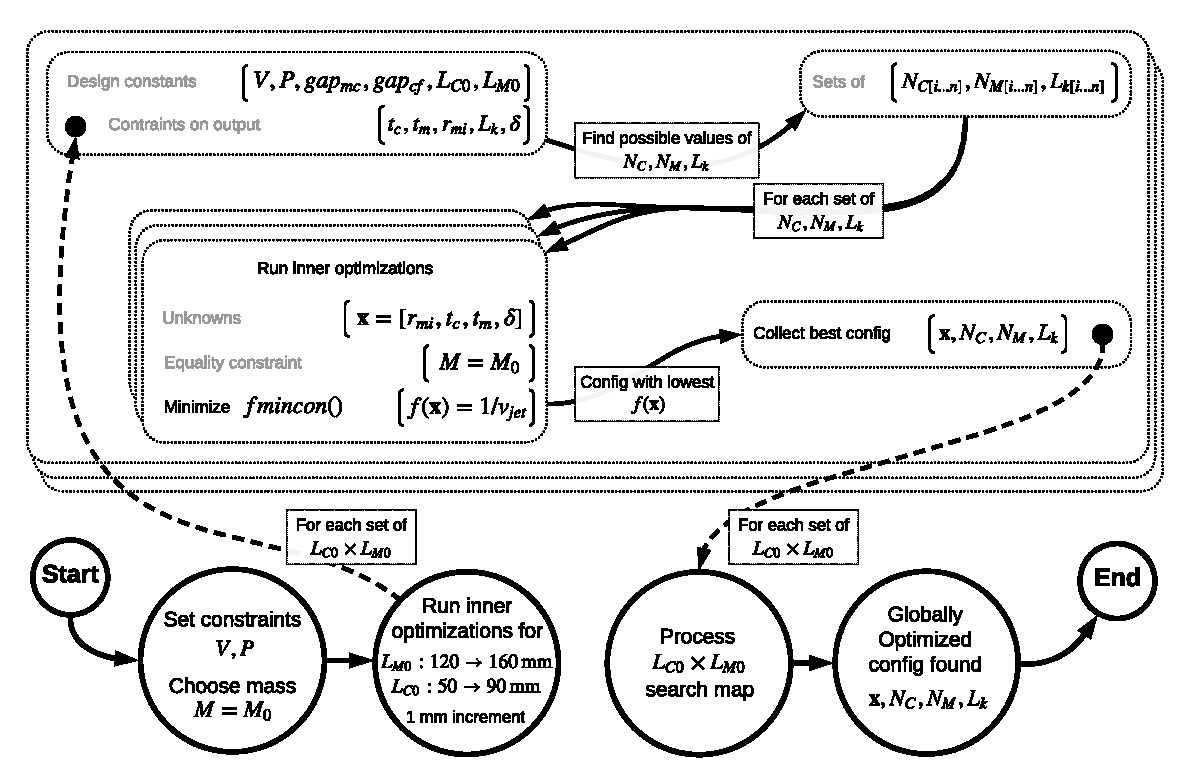
\includegraphics[width=5.8in]{chap3/images/HM_PMLSM_optimization.pdf}
              \caption{Summary of the top-level motor optimization algorithm and inner optimization routine. The algorithm uses motor specifications $V$, $P$, $M$ to determine the motor parameters $\textbf{x}=[r_{mi},t_c,t_m,\delta]$, $N_C$, $N_M$, $L_k$ at which the jet speed $v_{jet}$ can be maximized.}
              \label{fig:chapter/hm/top level optmization}
            \end{figure*}
            
            
            In summary, the outer optimization loop provides unique combinations of $L_{C0}$, $L_{M0}$, and $M_0$ to produce a set of possible $N_C$, as well as corresponding values of $N_M$ and $L_k$. At each point in the $L_{C0} \times L_{M0}$ space, multiple inner most optimizations will perform non-linear constraint optimization for unknown variable vector $\textbf{x}$:
            
            
            \begin{equation}
                \textbf{x} = \left[ r_{mi}, t_m, t_c, \delta\right]
                \label{eq:inner optimization x}
            \end{equation}
            
            
            Each inner optimization's aim is to find $\textbf{x}$ given $\left[N_C,N_M,L_k,M_0\right]$ from the outer optimization, and constants $\left[P,V\right]$ to maximize the jet speed $v_{jet}$ achieved where the same variable ranges in Table\,\ref{table:table_of_optimization_constraints_PMLSM} also applies: 
            
            
            \begin{equation}
                \begin{array}{rll}
                    \textbf{minimize}       & \small{objective\,\,function}     & f(\textbf{x})=\frac{1}{v_{jet}} \\
                    \textbf{subjected to}   & \small{equality\,\,constraint}    & h_1(\textbf{x})=M - M_0= 0
                \end{array}
                \label{eq:inner optimization for PMLSMs}
            \end{equation}
            
            
            
            With an unique set of $\left[\textbf{x}, N_C,N_M,L_k,M_0\right]$, the motor constant $K_m$ and motor mass $M$ can be found with the method outlined in Section\,\ref{Chapter:PMLSM design HM/electromagnetic model/hm solution}. Together with known power dissipation $P$, ampoule volume $V$, and water density $\rho_w$, the jet velocity $v_{jet}$ can be derived directly from Equation\,\ref{eq:power dissipation for PMLSMs}:
            
            
            \begin{equation}
                v_{jet} = \sqrt[4]{\frac{4P {K_m}^2 {L_S}^2}{\rho_w V^2}}
                \label{eq:v_jet}
            \end{equation}
            
            
            The inner optimization uses constrained nonlinear multi-variable optimization based on the interior point algorithm (MATLAB Optimization Toolbox) to minize the objective function in Equation\,\ref{eq:inner optimization for PMLSMs}. Upon finishing the inner optimizations for each pair $L_{C0} \times L_{M0}$, the control flow saves the best performing motor configuration and moves on to the next $L_{C0} \times L_{M0}$, obtains a next set of possible $N_C$ and so on. Fig.\,\ref{fig:chapter/hm/top level optmization} summarizes and illustrates both the outer and the inner optimization algorithms.
    
    
    % -----------------------------------------------------------------------------------
    % --- NEW SUB SECTION --- NEW SUB SECTION --- NEW SUB SECTION --- NEW SUB SECTION --- 
    % -----------------------------------------------------------------------------------
    \subsection{Results}                        \label{Chapter:PMLSM design HM/design optimization/results}
    
            
        The global optimization of \acs{PMLSM} for the problem described in Equation\,\ref{eq:outer optimization for PMLSMs} at different mass constraints $M_0=[325,350,375,400,425]\,\mathrm{g}$ are summarized in Table\,\ref{table:result for global optimization of PMLSM via HM method}.
            
            
        Taking an example for the global optimization of constraints set $P=1500\,\mathrm{W}$, $V=1\,\mathrm{mL}$, $gap_{mc}=1.2\,\mathrm{mm}$, $gap_{cf}=0.1\,\mathrm{mm}$, $M_0=325\,\mathrm{g}$ on the search space of $L_{M0}:120\,\mathrm{mm}\rightarrow 160\,\mathrm{mm}$, and $L_{C0}:50\,\mathrm{mm}\rightarrow 90\,\mathrm{mm}$, we found an under-hung motor with $N_C=4$, $N_M=12$, $L_k=26.5\,\mathrm{mm}$, $r_{mi}=2\,\mathrm{mm}$, $t_m=6.15\,\mathrm{mm}$, $t_c=3\,\mathrm{mm}$, $\delta=0.30$. The motor is able to theoretically produce $246.64\,\mathrm{N}$ at the rated power, which corresponds to a motor constant $K_m=6.37\,\mathrm{N/\sqrt{W}}$ and peak jet speed $v_{jet}=228.67\,\mathrm{m/s}$. The typical motor constant of \acsp{PMLSM} far exceed typical motor constant achieved by \acsp{VCM}\,\cite{ruddy2014}. The achievable jet speed $v_{jet}$ is beyond what is required for a successful needle free injection.
            
            
        According to Equation\,\ref{eq:power dissipation for PMLSMs}, and provided that $P$, $\rho_w$, $K_m$, $L_S$ are unchanged:
            
            
        \begin{equation}
            v_{jet}\propto\frac{1}{\sqrt{V}}
            \label{eq:v_jet and V}
        \end{equation}
            
            
        \begin{equation}
            V_{new}=\frac{v_{jet:old}}{v_{jet:new}}V_{old}
            \label{eq:v_jet and V ratio}
        \end{equation}
            
            
        If we now choose to adjust the ampoule cross-sectional area to reduce the peak jet speed $v_{jet}$ to $200\,\mathrm{m/s}$, the maximum volume $V$ of drug delivery can now be $V_{new}=1.31\,\mathrm{mL}$. 
            
            
        \begin{landscape}
            \begin{table}
                \renewcommand{\arraystretch}{1.2}
                \caption{Summary of motor design optimization values and performance}
                \label{table:result for global optimization of PMLSM via HM method}
                \centering
                \begin{tabular}{lllrrrrr}
                    \hline
                    \textbf{Params}     & \textbf{Description}                            & \textbf{Unit}           & $M_0=\mathbf{325\,g}$ & $\mathbf{350\,g}$ & $\mathbf{375\,g}$ & $\mathbf{400\,g}$ & $\mathbf{425\,g}$ \\
                    \hline
                    $P$        & Power dissipation in coil winding      & $\mathrm{kW}$  & $1.50$                & $1.50$            & $1.50$            & $1.50$            & $1.50$            \\
                    $V$        & Volume of ampoule                      & $\mathrm{mL}$  & $1.00$                & $1.00$            & $1.00$            & $1.00$            & $1.00$            \\
                    $gap_{mc}$ & Magnet and coil fixed gap              & $\mathrm{mm}$  & $1.20$                & $1.20$            & $1.20$            & $1.20$            & $1.20$            \\
                    $gap_{cf}$ & Coil and iron fixed gap                & $\mathrm{mm}$  & $0.10$                & $0.10$            & $0.10$            & $0.10$            & $0.10$            \\
                    \hline
                    $L_{C0:optim}$ & Constraint $L_C$ winding at global optimum & $\mathrm{mm}$        & $53.00$                       & $53.00$           & $53.00$           & $53.00$           & $53.00$           \\
                    $L_{M0:optim}$ & Constraint $L_C+L_S$ at global optimum        & $\mathrm{mm}$        & $160.00$                      & $160.00$          & $160.00$          & $160.00$          & $160.00$          \\
                    \hline
                    $r_{mi}$   & Magnet array inner radius              & $\mathrm{mm}$  & $2.00$                & $2.00$            & $2.00$            & $2.00$            & $2.00$            \\
                    $t_m$      & Magnet thickness                       & $\mathrm{mm}$  & $6.15$                & $6.35$            & $6.67$            & $6.99$            & $7.29$            \\
                    $t_c$      & Coil thickness                         & $\mathrm{mm}$  & $3.00$                & $3.00$            & $3.00$            & $3.00$            & $3.00$            \\
                    $\delta$   & Ratio of radial magnet vs. magnet pair &                & $0.30$                & $0.25$            & $0.26$            & $0.26$            & $0.27$            \\
                    $N_C$      & Number of half coil-poles              &                & $4$                   & $3$               & $3$               & $3$               & $3$               \\
                    $N_M$      & Number of half magnet-poles            &                & $12$                  & $9$               & $9$               & $9$               & $9$               \\
                    \hline
                    $t_f$      & Iron shell thickness                   & $\mathrm{mm}$  & $0.77$                        & $1.07$            & $1.12$            & $1.15$            & $1.19$    \\       
                    $L_k$      & Full pole length                       & $\mathrm{mm}$  & $26.50$               & $35.33$           & $35.33$           & $35.33$           & $35.33$           \\
                    $L_C$      & Length of coil array                   & $\mathrm{mm}$  & $53.00$               & $53.00$           & $53.00$           & $53.00$           & $53.00$           \\
                    $L_M$      & Length of magnet array                 & $\mathrm{mm}$  & $159.00$              & $159.00$          & $159.00$          & $159.00$          & $159.00$          \\
                    $L_S$      & Stroke length                          & $\mathrm{mm}$  & $106.00$              & $106.00$          & $106.00$          & $106.00$          & $106.00$          \\
                    \hline
                    $v_{jet}$  & Achievable jet speed                   & $\mathrm{m/s}$ & $228.67$              & $234.20$          & $239.84$          & $245.13$          & $250.10$         \\
                    $F$        & Force exerts on piston                 & $\mathrm{N}$         & $246.64$                      & $258.72$          & $271.35$          & $283.44$          & $295.06$          \\
                    $K_m$      & Motor constant                         & $\mathrm{N/\sqrt{W}}$ & $6.37$                        & $6.68$            & $7.01$            & $7.32$            & $7.62$           \\
                    \hline
                \end{tabular}
            \end{table}
        \end{landscape}
            
        \begin{figure*}[ht]
            \centering
            \subfloat[$M_0=325\,\mathrm{g}$. Global optimum found at $L_{C0}=53\,\mathrm{mm}$, $L_{C0}=160\,\mathrm{mm}$, $N_C=4$, and $N_M=12$.
            ]{
                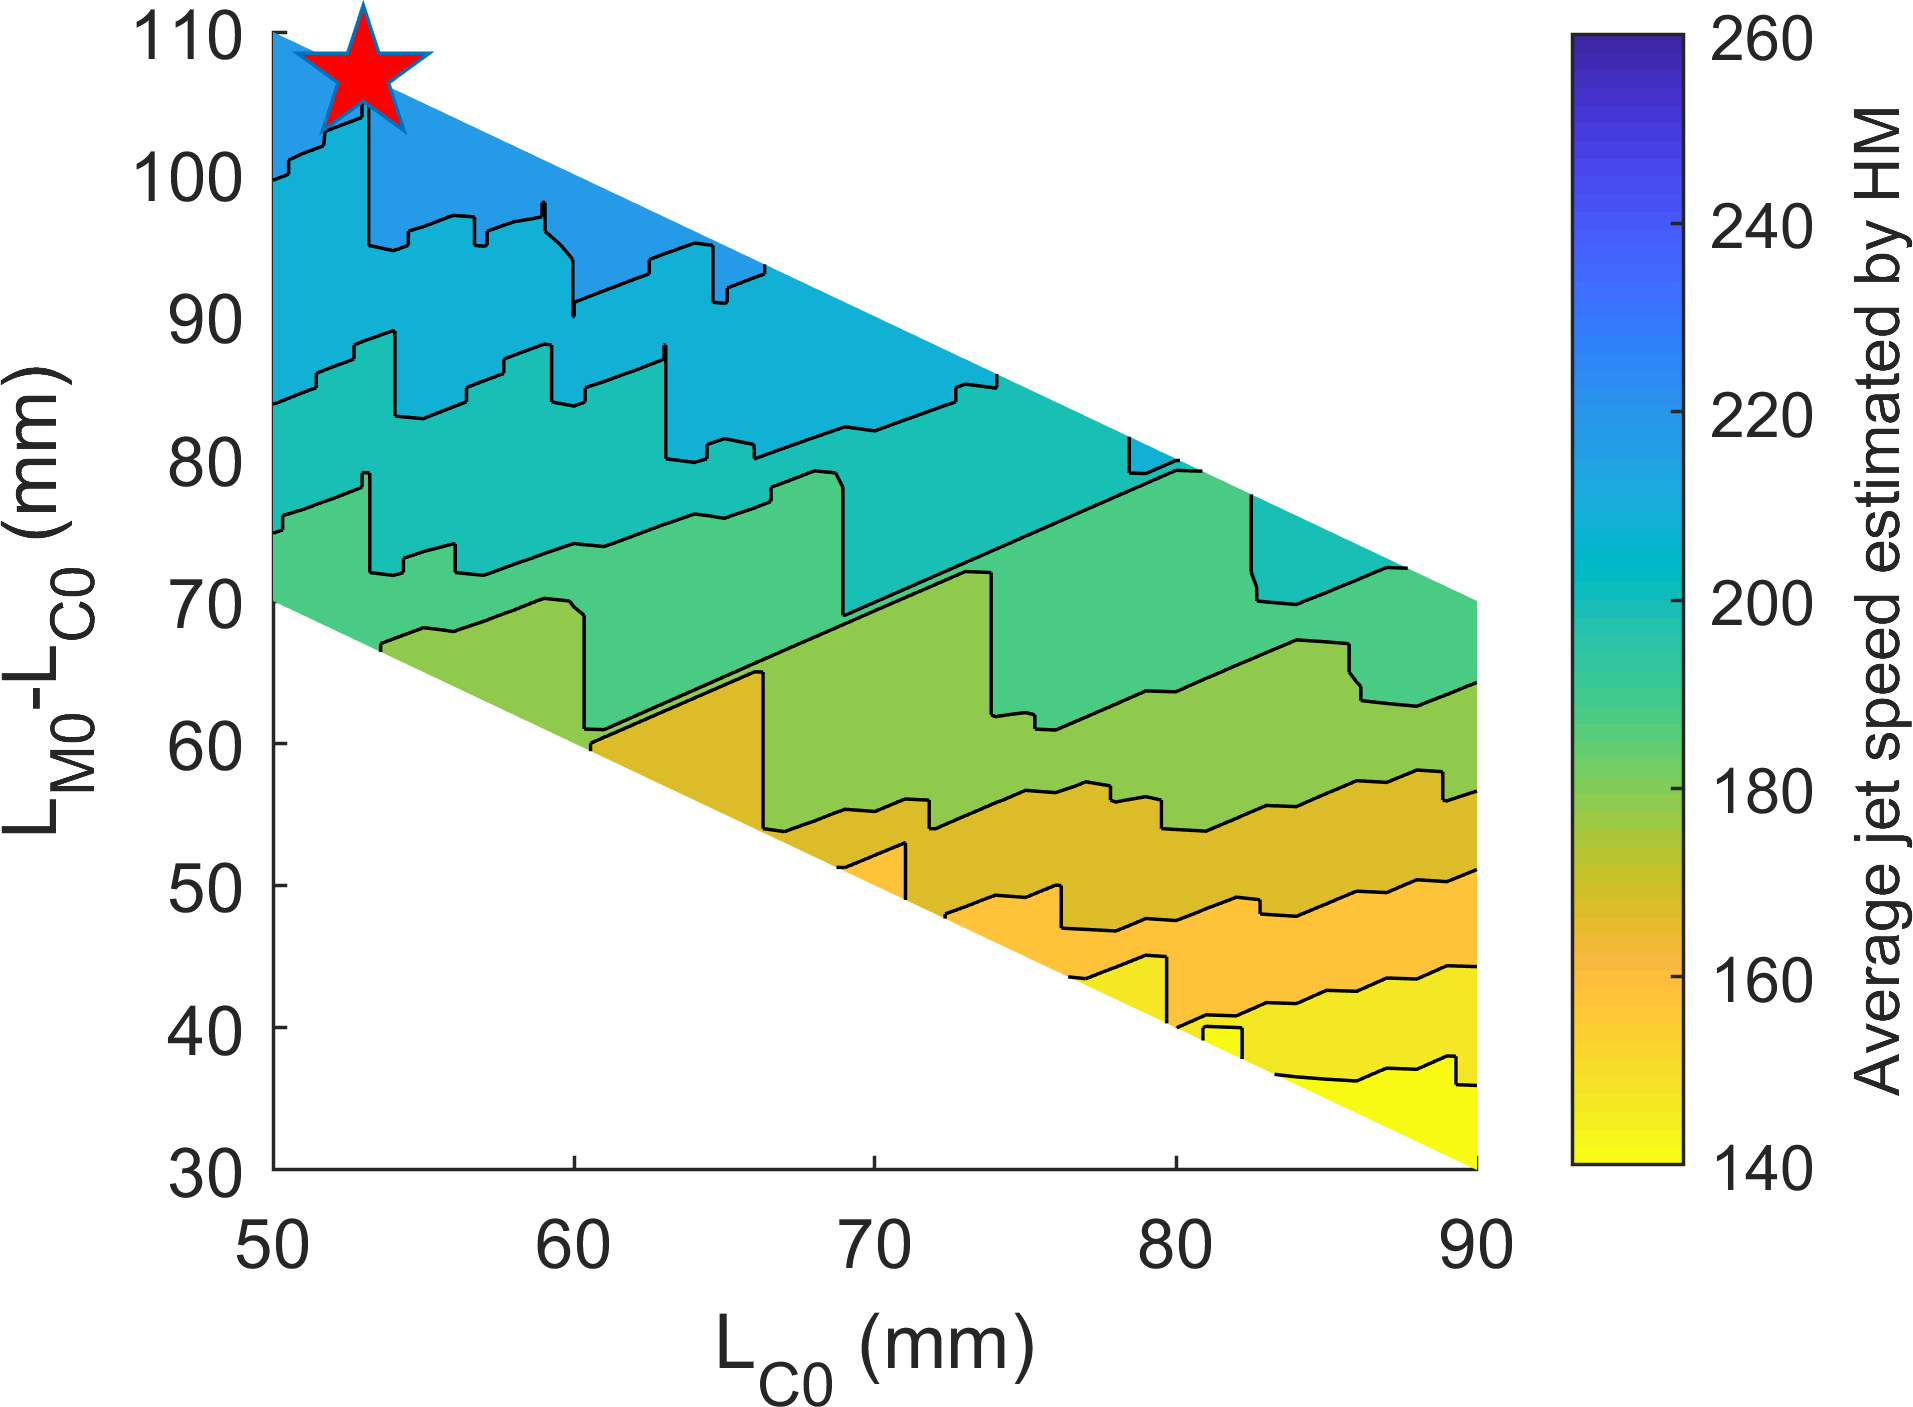
\includegraphics[width=0.45\textwidth]{chap3/images/PMLSM_HM_325g.png}
                \label{fig:chapter/hm/optimiization/325}
            }
            \qquad
            \subfloat[$M_0=350\,\mathrm{g}$ Global optimum found at $L_{C0}=53\,\mathrm{mm}$, $L_{C0}=160\,\mathrm{mm}$, $N_C=3$, and $N_M=9$.
            ]{
                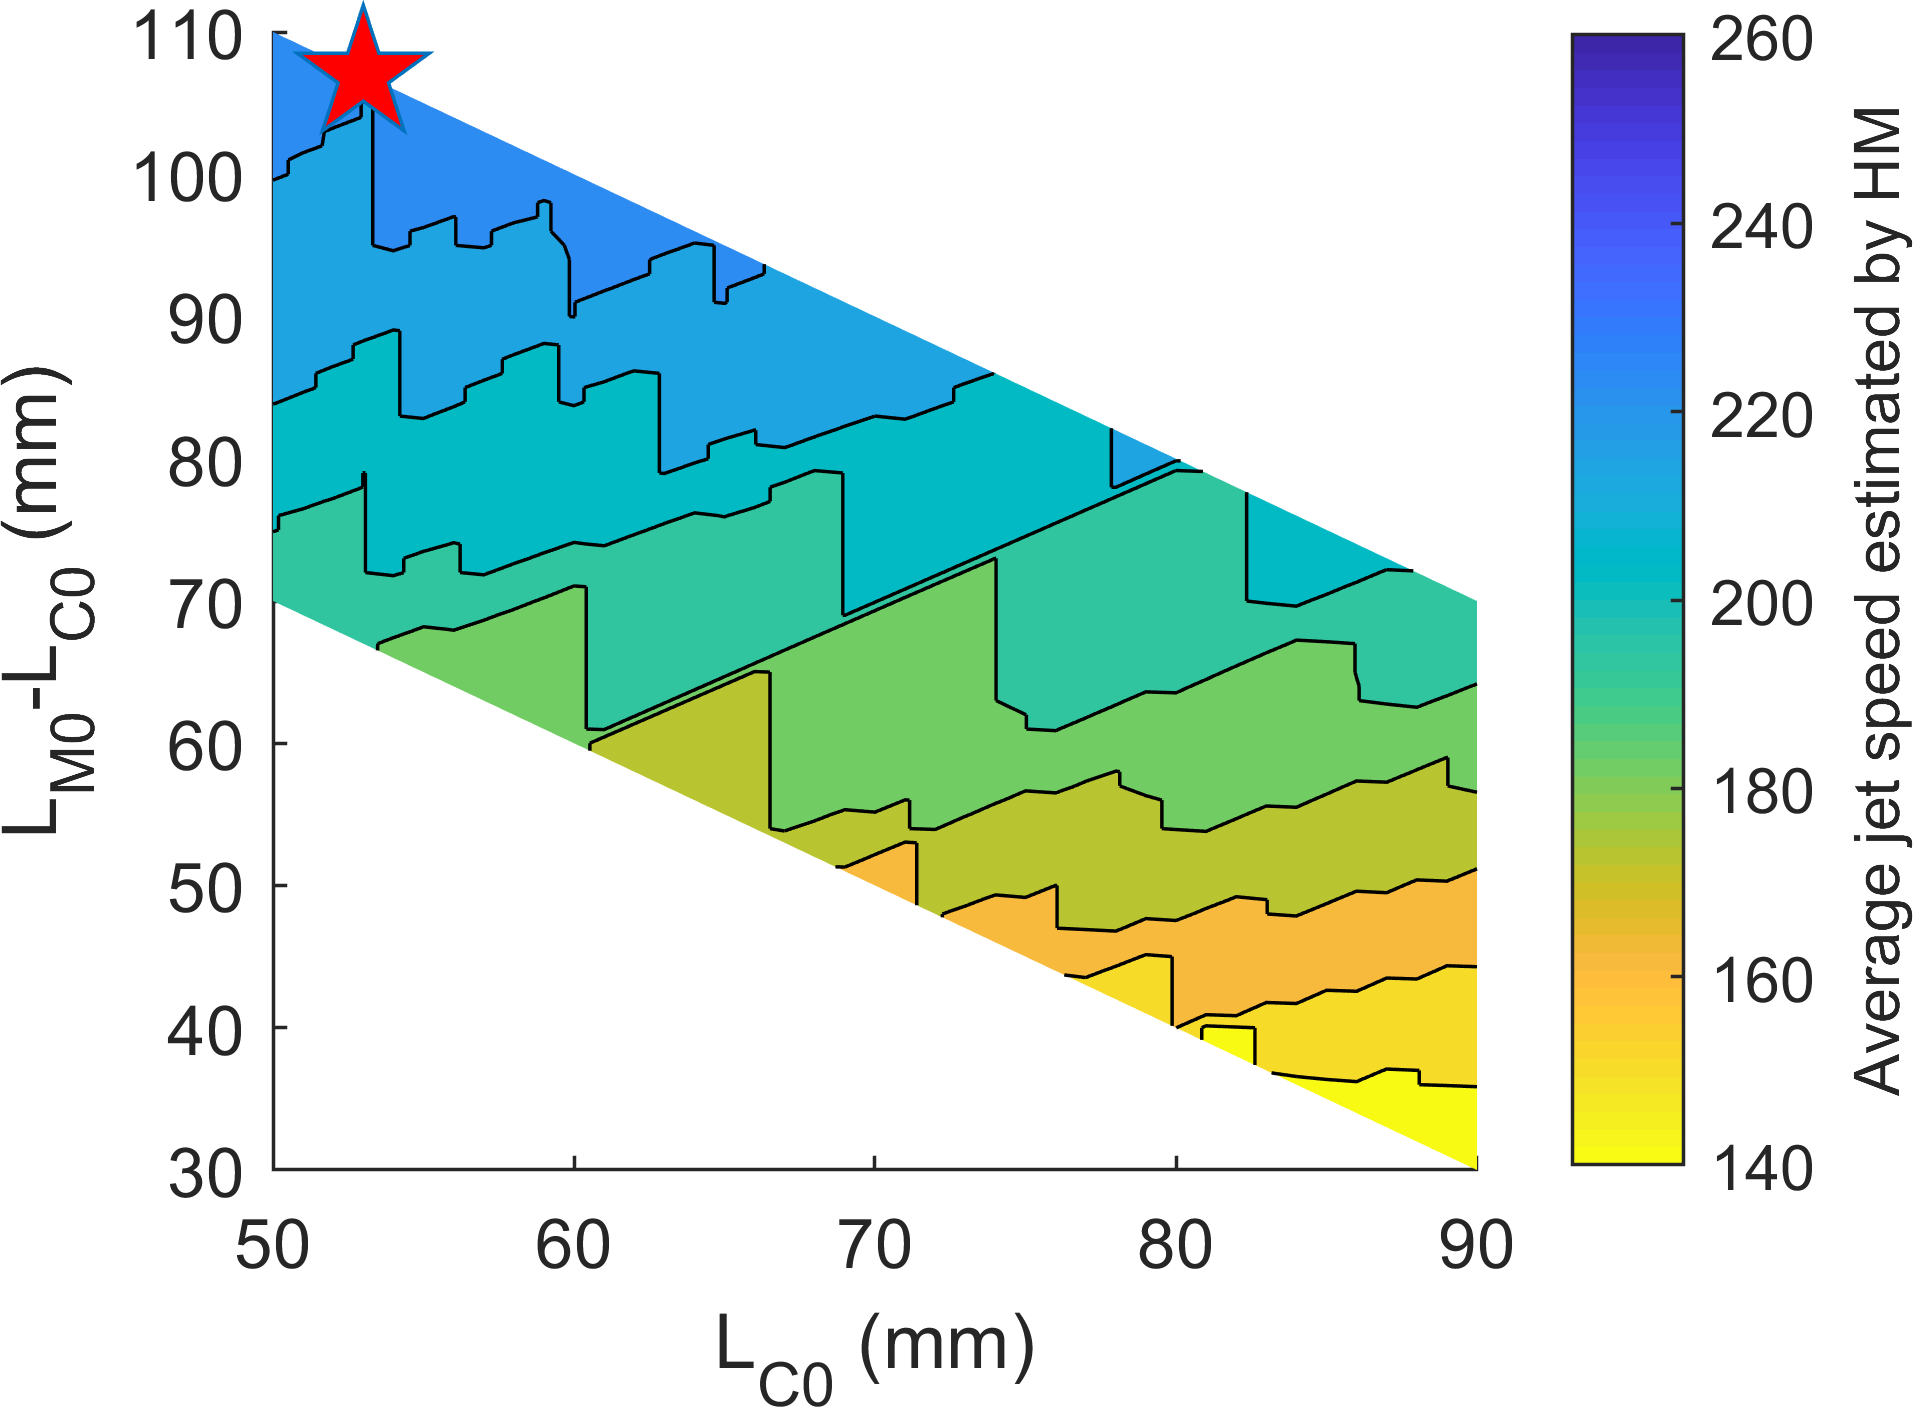
\includegraphics[width=0.45\textwidth]{chap3/images/PMLSM_HM_350g.png}
                \label{fig:chapter/hm/optimiization/350}
            }
            \\
            \subfloat[$M_0=375\,\mathrm{g}$. Global optimum found at $L_{C0}=53\,\mathrm{mm}$, $L_{C0}=160\,\mathrm{mm}$, $N_C=3$, and $N_M=9$.
            ]{
                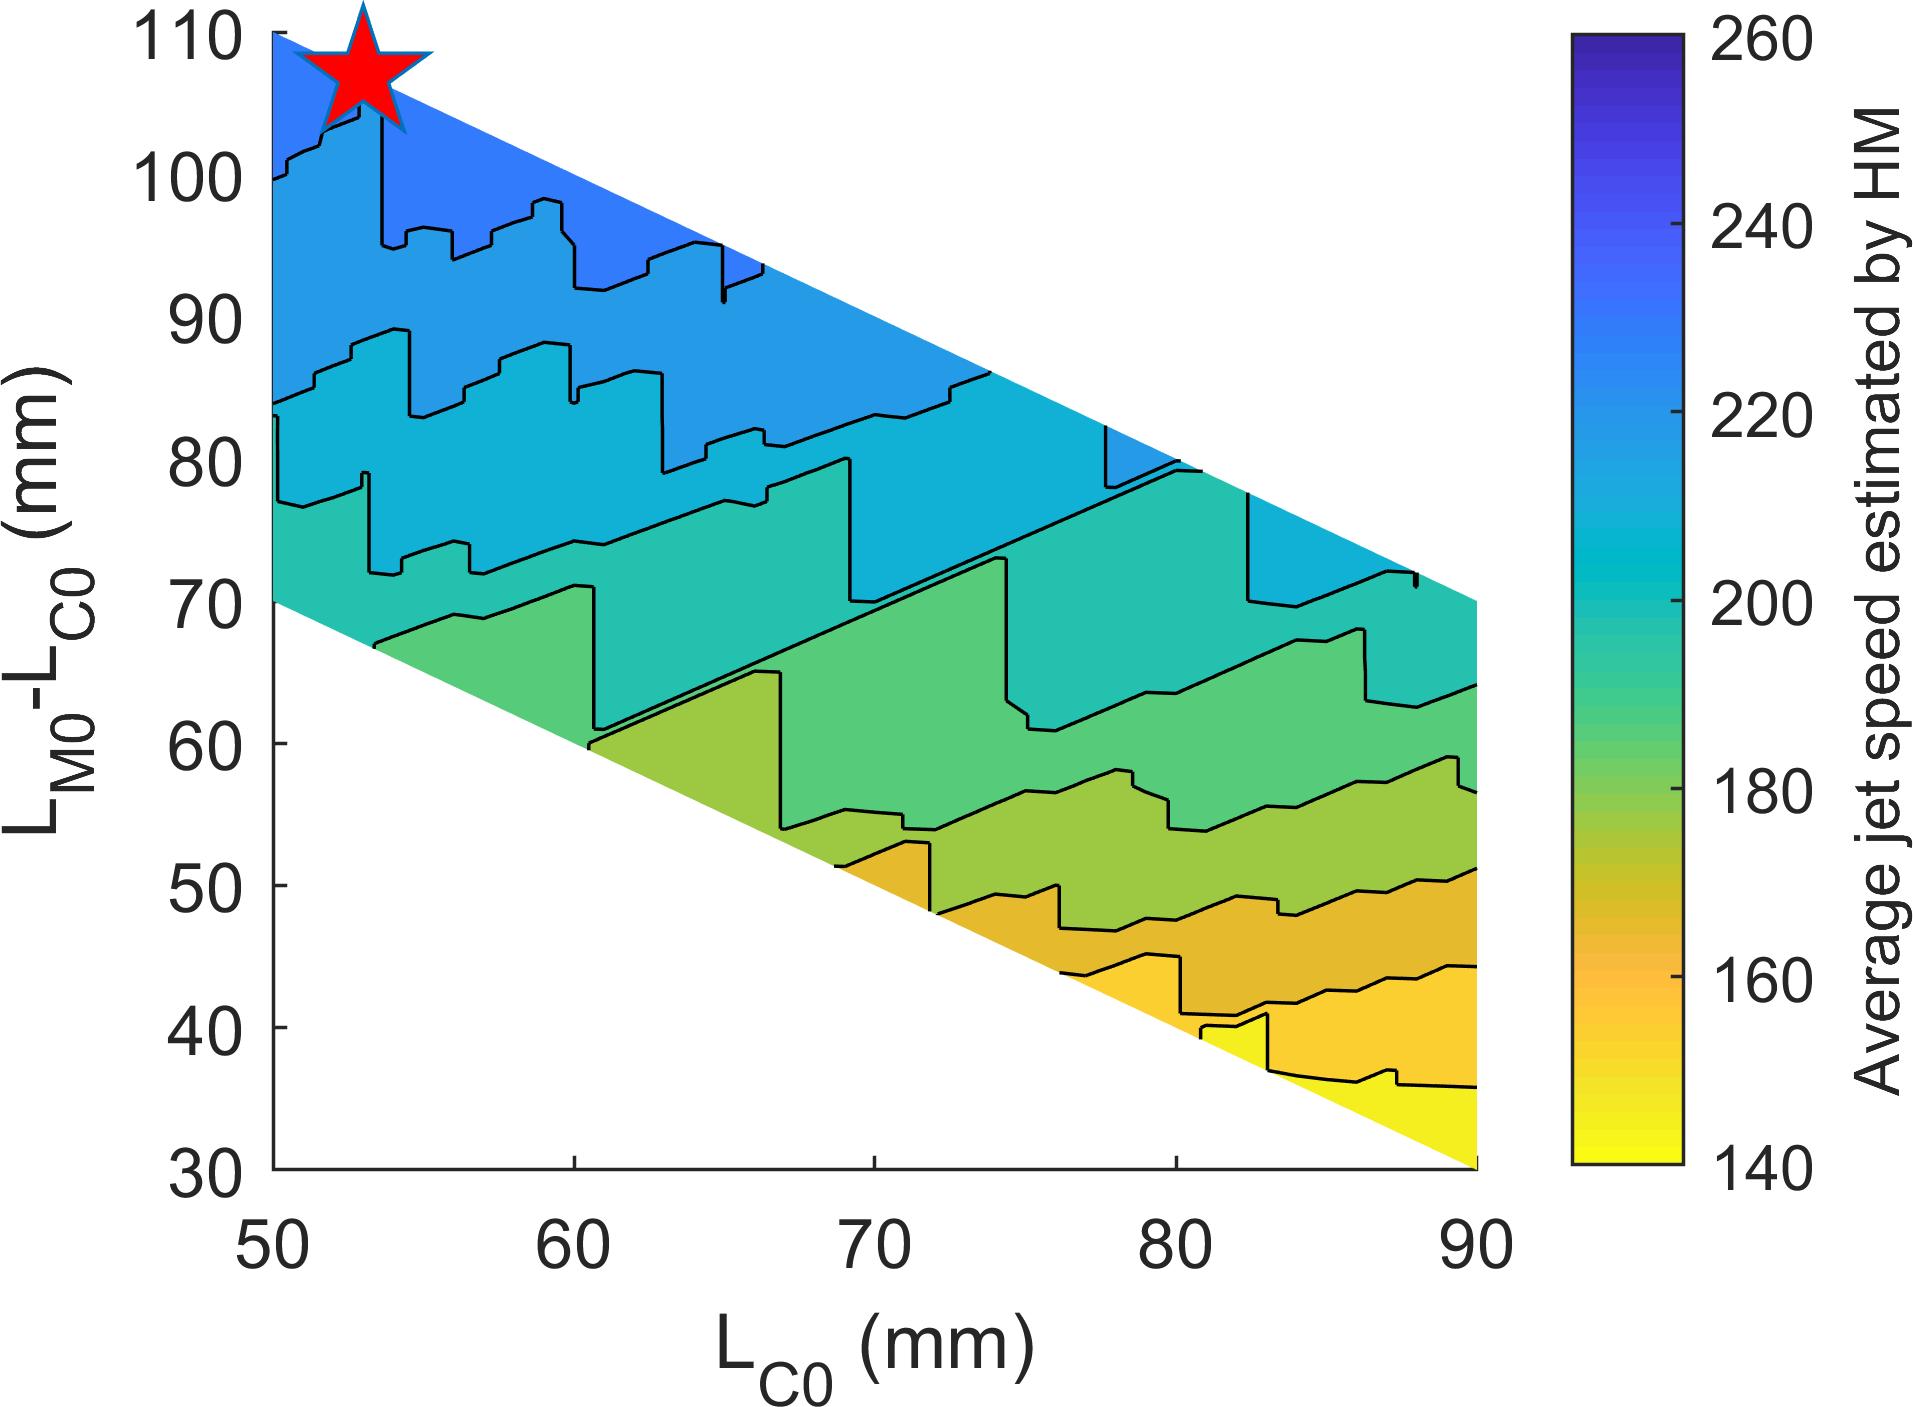
\includegraphics[width=0.45\textwidth]{chap3/images/PMLSM_HM_375g.png}
                \label{fig:chapter/hm/optimiization/375}
            }
            \qquad
            \subfloat[$M_0=400\,\mathrm{g}$. Global optimum found at $L_{C0}=53\,\mathrm{mm}$, $L_{C0}=160\,\mathrm{mm}$, $N_C=3$, and $N_M=9$.
            ]{
                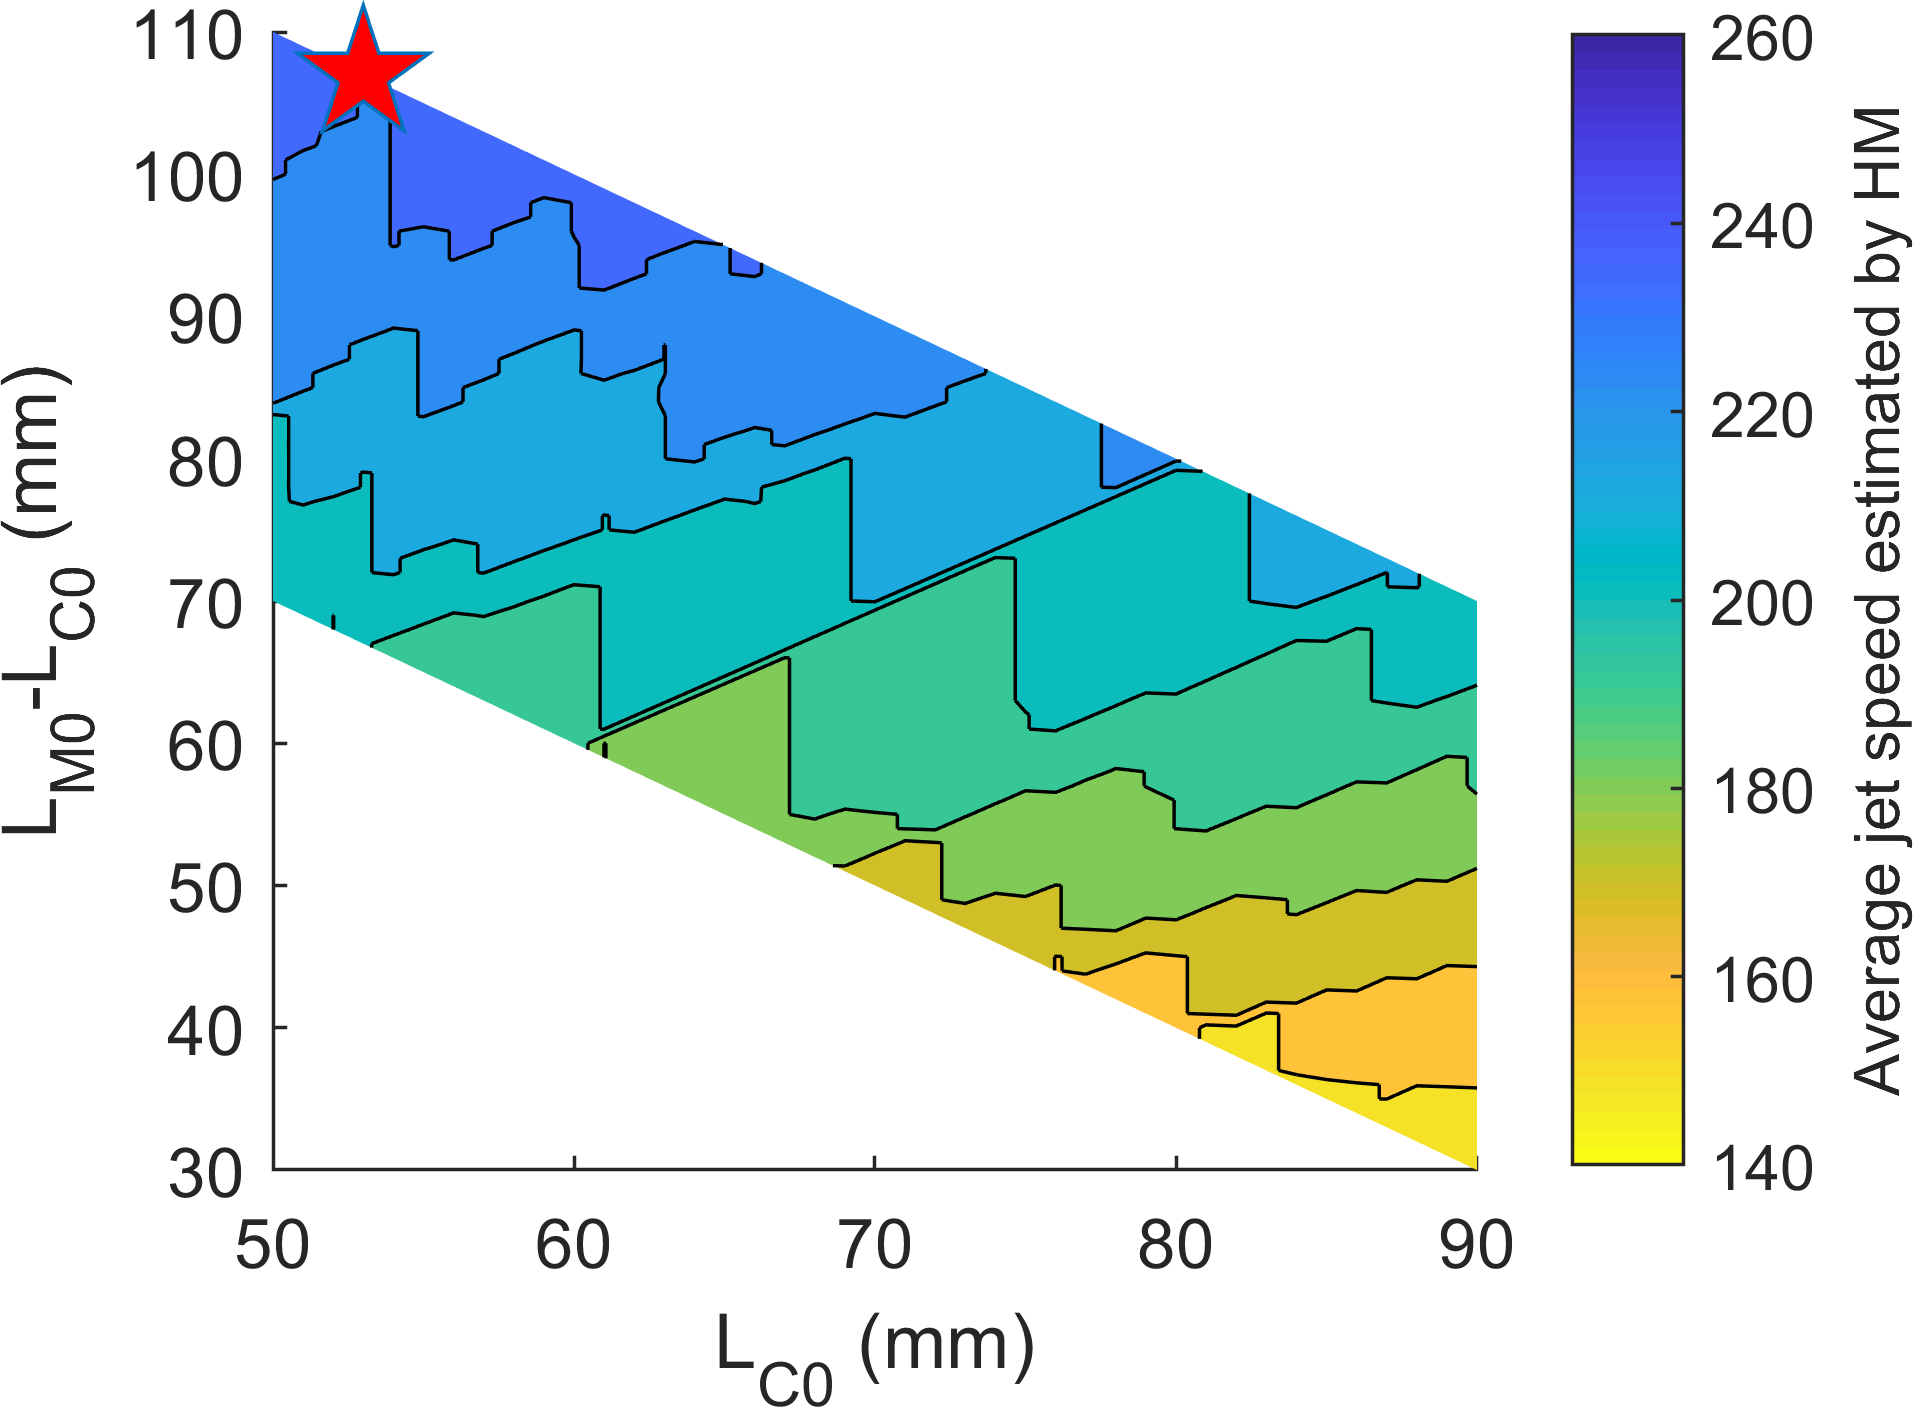
\includegraphics[width=0.45\textwidth]{chap3/images/PMLSM_HM_400g.png}
                \label{fig:chapter/hm/optimiization/400}
            }
            \\
            \subfloat[$M_0=425\,\mathrm{g}$. Global optimum found at $L_{C0}=53\,\mathrm{mm}$, $L_{C0}=160\,\mathrm{mm}$, $N_C=3$, and $N_M=9$.
            ]{
                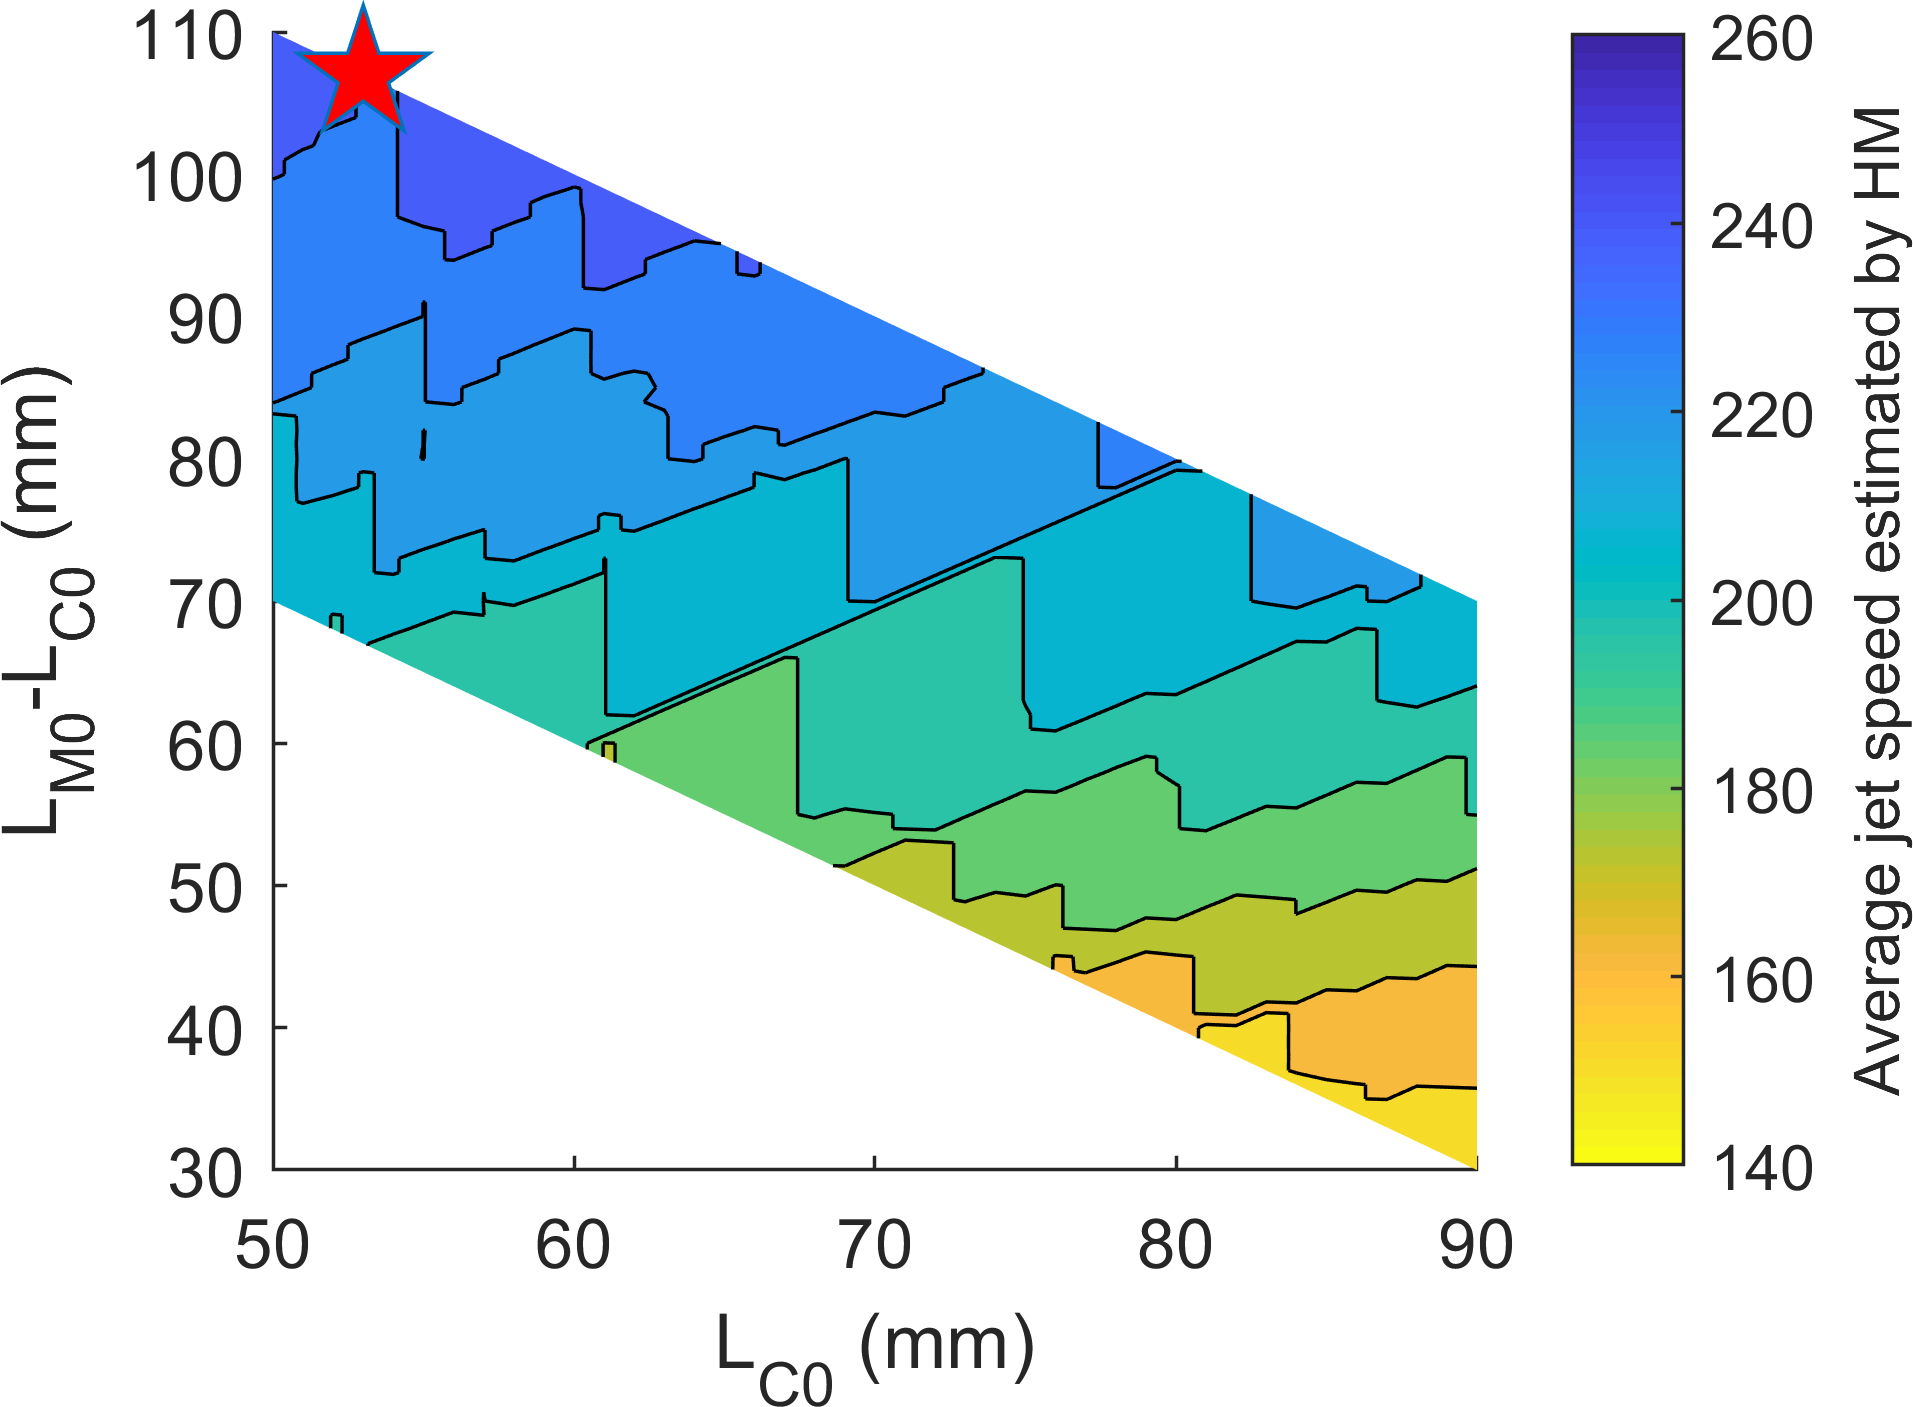
\includegraphics[width=0.45\textwidth]{chap3/images/PMLSM_HM_425g.png}
                \label{fig:chapter/hm/optimiization/425}
            }
            \\
            \caption{
                The global optimization plots of $v_{jet}$ for the search space $L_{M0}:120\,\mathrm{mm}\rightarrow 160\,\mathrm{mm} \times L_{C0}:50\,\mathrm{mm}\rightarrow 90\,\mathrm{mm}$ using $P=1500\,\mathrm{W}$, $V=1\,\mathrm{mL}$, $gap_{mc}=1.2\,\mathrm{mm}$, $gap_{cf}=0.1\,\mathrm{mm}$,  and $M_0$ of: (a) $325\,\mathrm{g}$, (b) $350\,\mathrm{g}$, (c) $375\,\mathrm{g}$, (d) $400\,\mathrm{g}$, and (e) $425\,\mathrm{g}$.
            }   \label{fig:chapter/hm/optimization search space result for differnt mass}
        \end{figure*}
            
        As expected, the more relaxed the mass constraint $M_0$, the higher the achievable jet speed $v_{jet}$ can be. Globally optimized motors at mass constraints $M_0$ of $350\,\mathrm{g}$, $350\,\mathrm{g}$, $375\,\mathrm{g}$, $400\,\mathrm{g}$, and $425\,\mathrm{g}$ can produce $v_{jet}$ of $229\,\mathrm{m/s}$, $234\,\mathrm{m/s}$, $240\,\mathrm{m/s}$, $245\,\mathrm{m/s}$, and $250\,\mathrm{m/s}$, respectively. Figure\,\ref{fig:chapter/hm/optimization search space result for differnt mass} provides global optimization plots of $v_{jet}$ for the search space $L_{M0}:120\,\mathrm{mm}\rightarrow 160\,\mathrm{mm} \times L_{C0}:50\,\mathrm{mm}\rightarrow 90\,\mathrm{mm}$ using $P=1500\,\mathrm{W}$, $V=1\,\mathrm{mL}$, $gap_{mc}=1.2\,\mathrm{mm}$, $gap_{cf}=0.1\,\mathrm{mm}$,  and $M_0=[325,350,375,400,425]\,\mathrm{g}$. Although the 2D contour patterns appear similar across the different plots, the color shade gradually gets darker with easier mass constraints $M_0$, indicating an increase in the motor performance.
            

    % ===================================================================================================
    % === NEW SECTION === NEW SECTION === NEW SECTION === NEW SECTION === NEW SECTION === NEW SECTION ===
    % ===================================================================================================
    \section{Discussion}                            \label{Chapter:PMLSM design HM/discussion}
    
        
        To summarize, this chapter provides a semi-analytical solution for the electromagnetic model of slotless tubular \acsp{PMLSM} (Section\,\ref{Chapter:PMLSM design HM/electromagnetic model}), an efficient optimization scheme for a fixed motor mass at a given power dissipation (Section\,\ref{Chapter:PMLSM design HM/design optimization/optimization formulation}). Utilizing these modeling and optimization methodologies, we performed a case study and found a globally optimized motor configurations for \acs{NFJI} under different mass constraints (Section\,\ref{Chapter:PMLSM design HM/design optimization/optimization formulation}). The optimized motor configuration for these requirements is summarized in Table~\ref{table:result for global optimization of PMLSM via HM method}. Most importantly, this work was able to confirm that \acsp{PMLSM} readily outperform \acsp{VCM} in \acs{NFJI} applications: being able deliver more volume with far less energy.
        
        
        The optimization benchmark optimization specification established in Section\,\ref{Chapter:PMLSM design HM/design optimization/design citeria} is especially important, and will be reused in accessing and comparing other types of \acsp{LSDDM} in the later Chapter\,\ref{Chapter:PMLSM design RSM}.
        
        